\documentclass[tikz,border=4pt]{standalone}
\usepackage[utf8]{inputenc}
\usepackage[T1]{fontenc}
\usepackage{amsmath,amssymb}
\usepackage{tikz}
\usetikzlibrary{arrows.meta,positioning,shapes.geometric,fit,calc,backgrounds,decorations.pathreplacing}
\definecolor{granate}{RGB}{138,0,0}
\definecolor{pizarra}{RGB}{43,58,85}
\definecolor{verdee}{RGB}{46,125,50}
\definecolor{ambar}{RGB}{242,169,0}
\definecolor{grisb}{RGB}{158,158,158}
\definecolor{grisc}{RGB}{238,238,236}
\definecolor{celeste}{RGB}{42,120,214}
\tikzset{
  bloque/.style={draw=pizarra,fill=white,rounded corners=3pt,thick,align=center,font=\sffamily\small,inner sep=5pt,minimum height=1.0cm},
  alcance/.style={bloque,fill=granate!10,draw=granate,very thick},
  fuera/.style={bloque,fill=grisc,draw=grisb,dashed,text=black!55},
  flecha/.style={-{Stealth[length=2.6mm]},thick,draw=pizarra},
  flechaf/.style={-{Stealth[length=2.6mm]},thick,draw=grisb,dashed},
  etiq/.style={font=\sffamily\scriptsize,text=pizarra,align=center}
}

\begin{document}
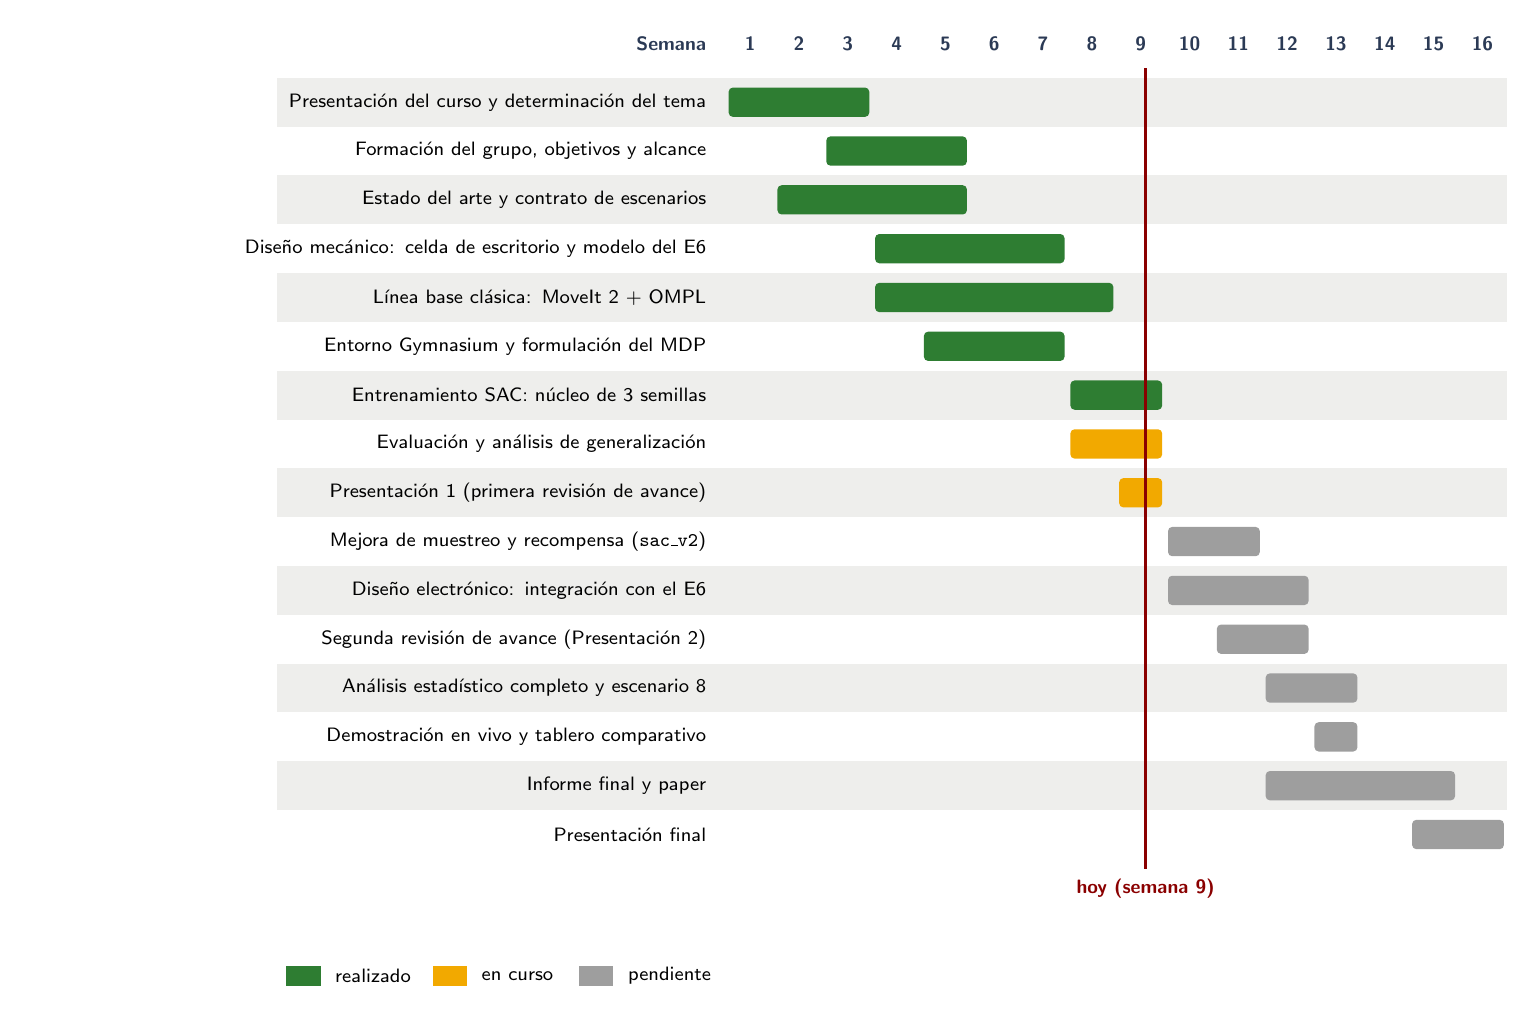
\begin{tikzpicture}[x=0.62cm,y=-0.62cm,font=\sffamily\scriptsize]
\def\hoy{8.6}
\foreach \w in {1,...,16}{\node[font=\sffamily\scriptsize\bfseries,text=pizarra] at (\w-0.5,-0.7) {\w};}
\node[anchor=east,font=\sffamily\scriptsize\bfseries,text=pizarra] at (-0.2,-0.7) {Semana};
\newcounter{fila}\setcounter{fila}{0}
\newcommand{\act}[4]{%
  \stepcounter{fila}%
  \pgfmathtruncatemacro{\r}{\value{fila}}%
  \ifodd\r\fill[grisc] (-9.2,\r-1) rectangle (16,\r);\fi
  \node[anchor=east,text width=8.5cm,align=right] at (-0.2,\r-0.5) {#1};
  \fill[#4,rounded corners=1.5pt] (#2-1+0.06,\r-0.8) rectangle (#3-0.06,\r-0.2);}
\act{Presentación del curso y determinación del tema}{1}{3}{verdee}
\act{Formación del grupo, objetivos y alcance}{3}{5}{verdee}
\act{Estado del arte y contrato de escenarios}{2}{5}{verdee}
\act{Diseño mecánico: celda de escritorio y modelo del E6}{4}{7}{verdee}
\act{Línea base clásica: MoveIt 2 + OMPL}{4}{8}{verdee}
\act{Entorno Gymnasium y formulación del MDP}{5}{7}{verdee}
\act{Entrenamiento SAC: núcleo de 3 semillas}{8}{9}{verdee}
\act{Evaluación y análisis de generalización}{8}{9}{ambar}
\act{Presentación 1 (primera revisión de avance)}{9}{9}{ambar}
\act{Mejora de muestreo y recompensa (\texttt{sac\_v2})}{10}{11}{grisb}
\act{Diseño electrónico: integración con el E6}{10}{12}{grisb}
\act{Segunda revisión de avance (Presentación 2)}{11}{12}{grisb}
\act{Análisis estadístico completo y escenario 8}{12}{13}{grisb}
\act{Demostración en vivo y tablero comparativo}{13}{13}{grisb}
\act{Informe final y paper}{12}{15}{grisb}
\act{Presentación final}{15}{16}{grisb}
\draw[granate,very thick] (\hoy,-0.2) -- (\hoy,16.2);
\node[text=granate,font=\sffamily\scriptsize\bfseries] at (\hoy,16.6) {hoy (semana 9)};
\begin{scope}[shift={(-9.0,18.2)}]
\fill[verdee] (0,0) rectangle (.7,.4); \node[anchor=west] at (.8,.2) {realizado};
\fill[ambar] (3,0) rectangle (3.7,.4); \node[anchor=west] at (3.8,.2) {en curso};
\fill[grisb] (6,0) rectangle (6.7,.4); \node[anchor=west] at (6.8,.2) {pendiente};
\end{scope}
\end{tikzpicture}
\end{document}
